\documentclass[10pt,a4paper]{report}
\usepackage[utf8]{inputenc}
\usepackage[spanish]{babel}
\usepackage{amsmath}
\usepackage{amsfonts}
\usepackage{amssymb}
\usepackage{graphicx}
\usepackage{fancyhdr}
\usepackage{float}
\usepackage{color}
\usepackage{mcode}
\usepackage[left=2cm,right=2cm,top=2cm,bottom=2cm]{geometry}

\author{Alamilla Ortiz Cesar Alejandro\\Cabrera López Óscar Emilio\\Castillo Cruz Heriberto\\Cuevas Mondragón Ricardo\\Equipo 9}
\title{Serie 1}

\pagestyle{fancy}
\fancyhf{}
\lhead[]{}
\chead[]{}
\rfoot{\thepage}
\lfoot[]{}
\cfoot[]{}

\renewcommand\headrule
{{\color[RGB]{98,36,35}%
    \hrule height 2pt
    width\headwidth
    \vspace{1.3pt}%
    \hrule height 1pt
    width\headwidth
  }}
  \addto\captionsspanish{\def\tablename{Tabla}}%imprime Tabla en lugar de Cuadro
  %%
  \spanishdecimal{.}


\begin{document}
\thispagestyle{fancy}
\maketitle
\tableofcontents
\newpage
\setcounter{chapter}{1}

\section[Ejercicio 1]{Ejercicio 1}

Obtenga una expresión en términos de funciones singulares la señal de tiempo continuo x(t) mostrada en la figura 1. Utilice la parábola $u_{-3}(t)$.\\

\begin{figure}[H]
  \begin{center}
    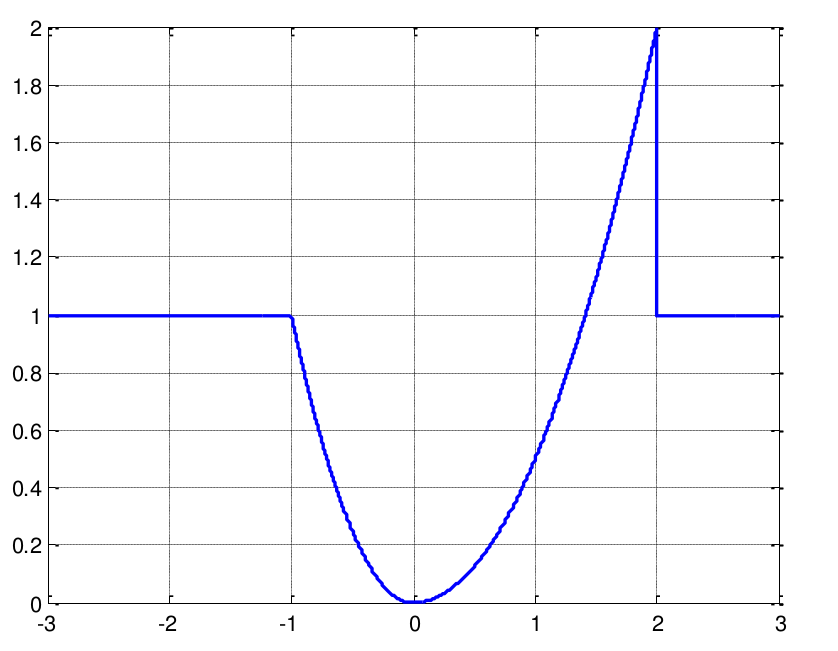
\includegraphics[width=0.6\textwidth]{SignalEjemplo}
    \caption{Ejercicio 1}
    \label{fig:Ejercicio 1}
  \end{center}
\end{figure}



\begin{figure}[H]
\centering
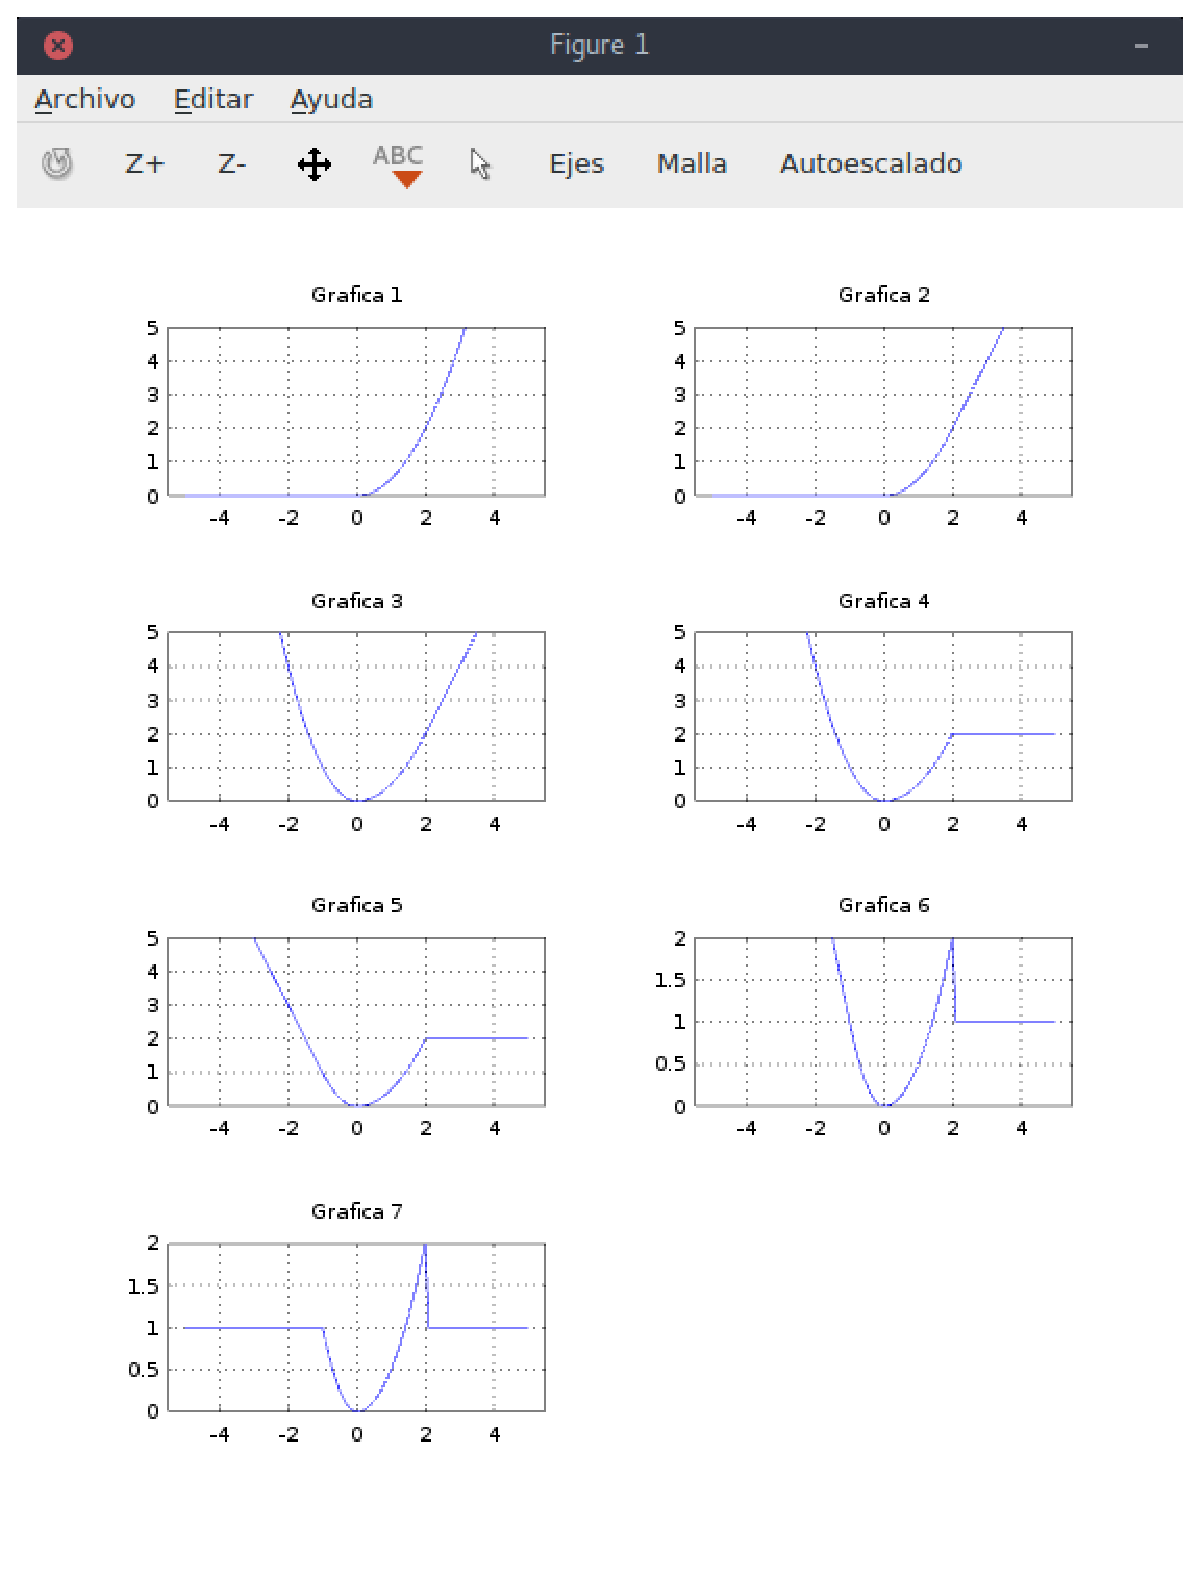
\includegraphics[width=0.6\textwidth]{SignalGraphic}
\caption{Aproximaciones a la señal}
\label{fig:SignalGraphic}
\end{figure}


\section{Ejercicio 2}
Si x(t) es la que obtuvo en el Ejercicio 1, obtenga las siguientes señales:\\
a) x(t/4)\\

\begin{figure}[H]
\centering
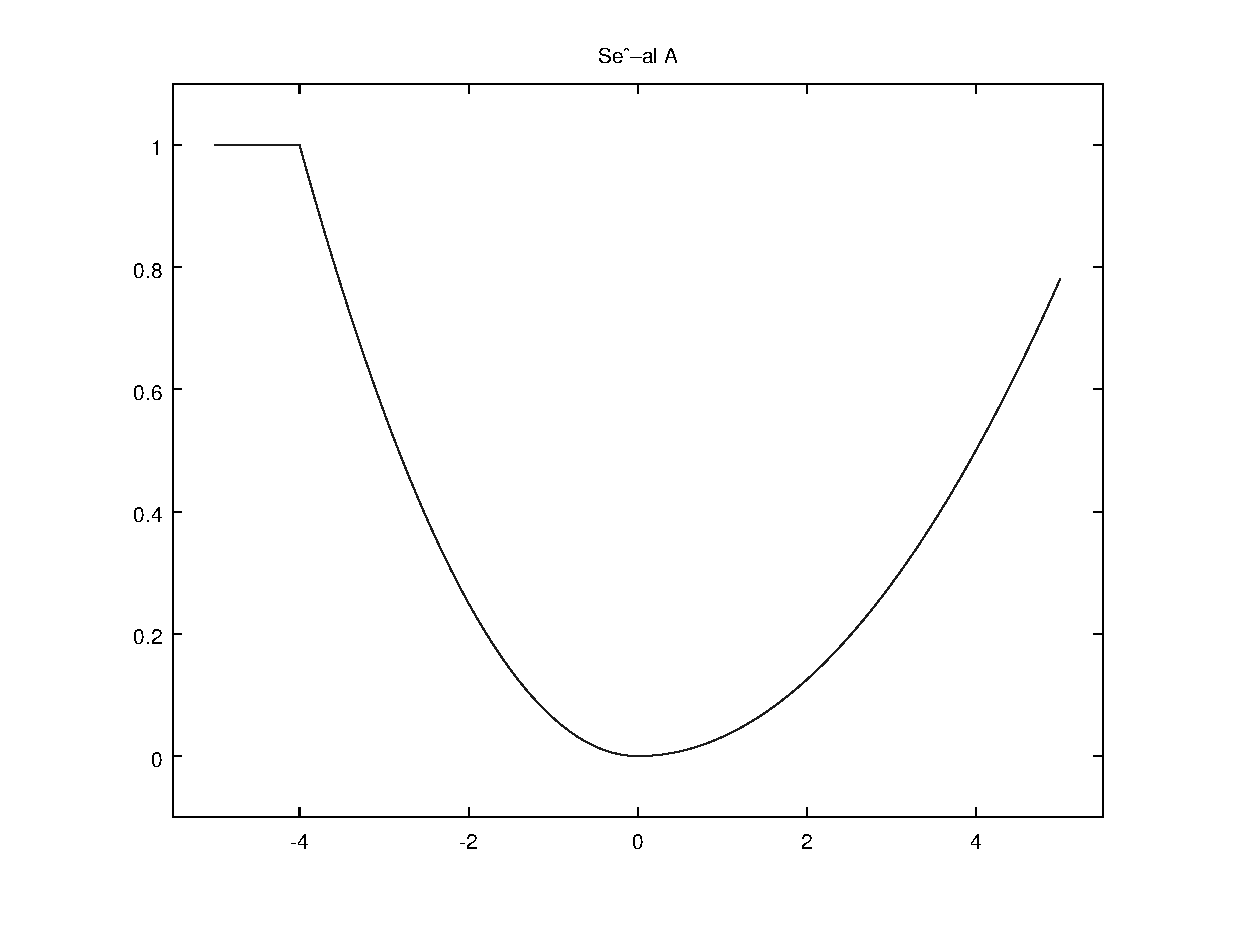
\includegraphics[width=0.6\textwidth]{SignalA}
\caption{Señal A}
\label{fig:SignalA}
\end{figure}

b) x(2t-1/4)\\

\begin{figure}[H]
\centering
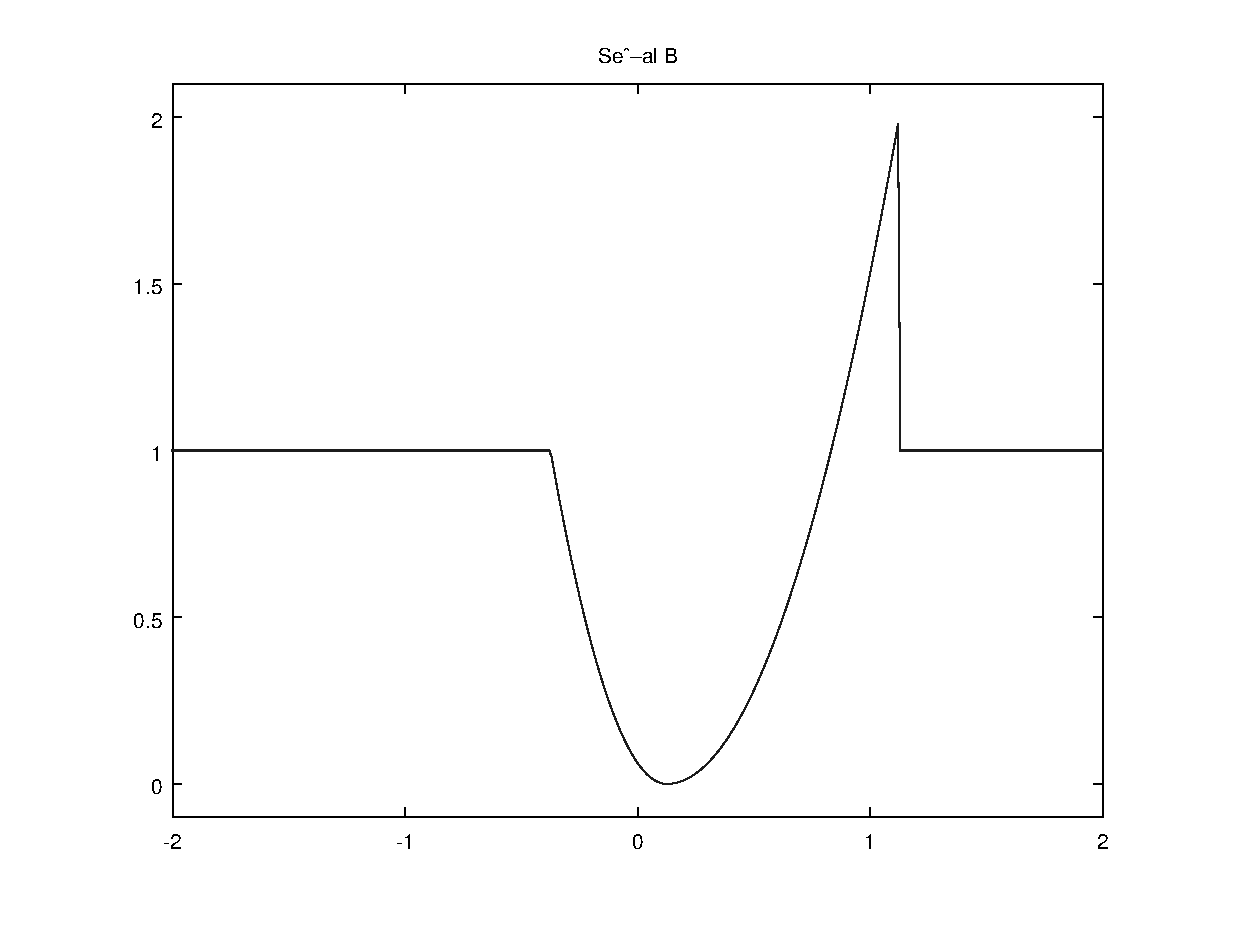
\includegraphics[width=0.6\textwidth]{SignalB}
\caption{Señal B}
\label{fig:SignalB}
\end{figure}

c) x(-t/4-1)\\

\begin{figure}[H]
\centering
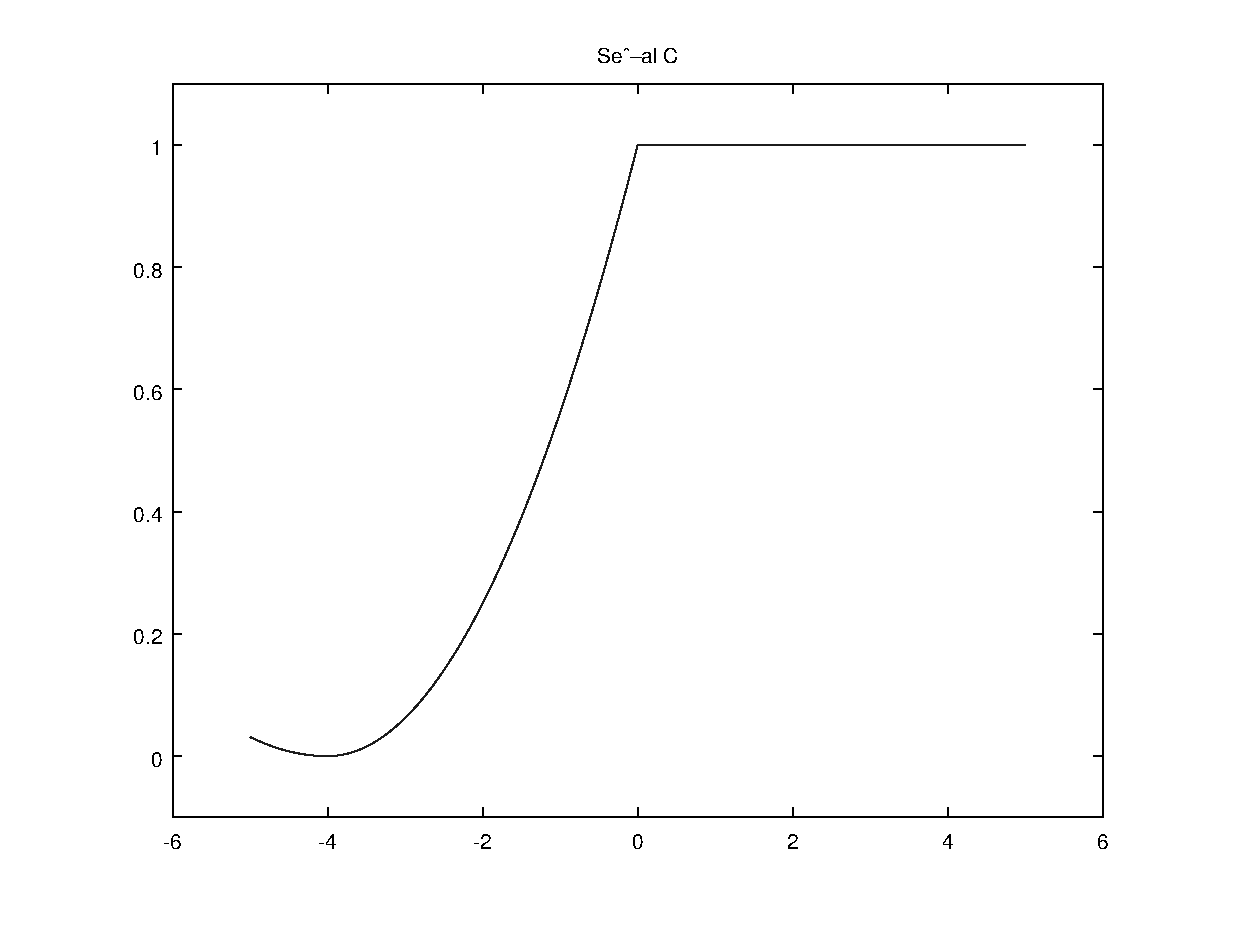
\includegraphics[width=0.6\textwidth]{SignalC}
\caption{Señal C}
\label{fig:SignalC}
\end{figure}

d) x(t/4+1/4)\\

\begin{figure}[H]
\centering
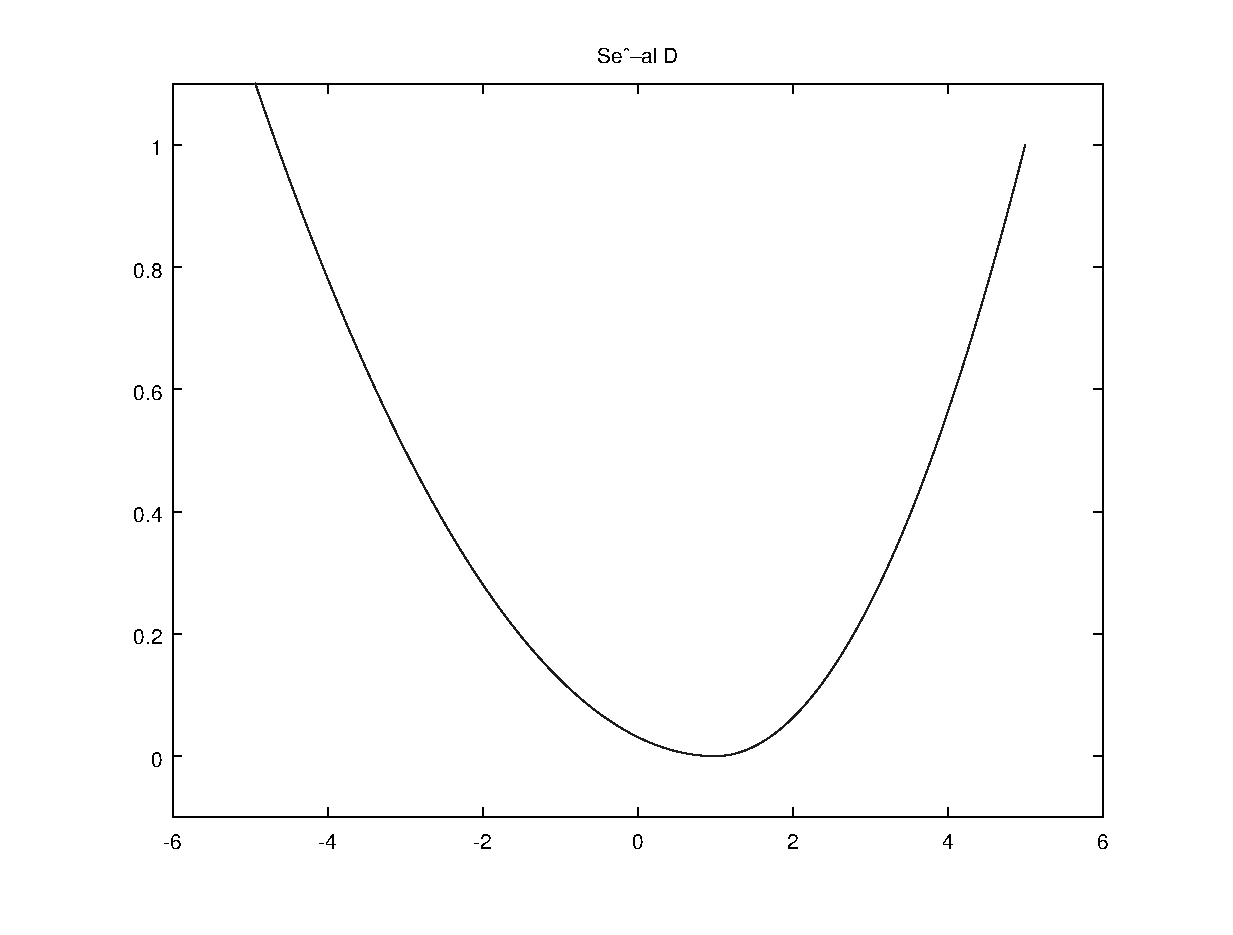
\includegraphics[width=0.6\textwidth]{SignalD}
\caption{Señal D}
\label{fig:SignalD}
\end{figure}



\section{Ejercicio 4}
Determine si los siguientes sistemas de tiempo continuo son o no lineales, variantes en el tiempo, causales, con memoria y estables. Justifique su respuesta.
%%
\begin{itemize}
\item \begin{equation}
 y(n)=
 \left\{
  \begin{aligned}
   1\quad n>=0\\
   0\quad n<0\
  \end{aligned}
 \right.
\label{escunit}
\end{equation}
%%
Este no es el modelo de un sistema ya que no relaciona la entrada con la salida.
\item  \begin{equation*}
y(t)=sen(x(t+1))
\end{equation*}
* Lineal o no lineal\\

   x1(t) = y1(t)= sen (x1(t+1))\\
   x2(t) = y2(t)= sen (x2(t+1))\\
   x3(t) = x1(t)+x2(t) = y3(t)=sen(x3(t+1))\\
                         y3(t)=sen(x1(t+1)+x2(t+1))\\

 NO LINEAL\\

* Variante o invariante en el tiempo\\

  y(t-t0)=sen(x(t-t0+1)) ... A esto se debe llegar\\
  Proponer: x1(t)=x(t-t0) --- y1(t)=sen(x1(t+1))\\
  y1(t)=sen(x(t+1-t0))\\

  INVARIANTE EN EL TIEMPO\\

* Causalidad\\

y(0)=sen(x(1))\\
y(-1)=sen(x(0))\\
y(1)=sen(x(2))\\

NO CAUSAL O ANTICIPATIVO, porque depende de valores futuros. \\

* Memoria\\

CON MEMORIA, por que depende de valores futuros.\\

* Estabilidad\\
ESTABLE, ya que al probar con una señal como el escalón, la entrada y la salida es acotada.\\

\end{itemize}

\section{Ejercicio 5}

Evalúe las siguientes integrales:
\begin{equation}
y(t)=\int_{-\infty }^{\infty }[3\delta (t)+e^{-(t-1)}\delta (t)+cos(2\pi t)\dot{\delta} (t)+e^{-t}\ddot{\delta }(t) ]dt
\end{equation}

\begin{equation}
y(t)=\int_{0}^{\infty }e^{-(t-1)}\delta (t+10)dt
\end{equation}\\

Para la primera ecuación tenemos que gracias a la propiedad de      linealidad podemos realizar esta descomposición:\\

\begin{equation}
y(t)=3\int_{-\infty }^{\infty }\delta (t)dt+\int_{-\infty }^{\infty }e^{-(t-1)}\delta (t)dt+\int_{-\infty }^{\infty }cos(2\pi t)\dot{\delta (t)}dt+\int_{-\infty }^{\infty }e^{-t}\ddot{\delta}(t)dt
\end{equation}\\
Sabiendo que la transformada de Laplace de delta de Dirac es:
\begin{equation}
L\left \{ \delta \left ( t \right ) \right \}=1
\end{equation}\\
Y que:
\begin{equation}
L\left \{ f(t)\delta (t-a) \right \}=\int_{0 }^{\infty }e^{-st}f(t)\delta (t-a)dt=e^{-as}f(a)
\end{equation}\\
Basándonos en esos conceptos ya nos es posible operar\\
Utilizando la transformada de Laplace
\begin{equation}
3L\left \{ \delta (t) \right \}=3\ast 1=3
\end{equation}\\
Aplicando la transformada al otro termino quedaría:
\begin{equation}
L\left \{ e^{-(t-1)}\delta (t) \right \}
\end{equation}\\
Ayudándonos de la ecuación numero 5 tenemos que a=0 por lo tanto:\\
\begin{equation}
e^{-as}\cdot f(a)=e^{-0s}\cdot e^{-(0-1)}=e^{o}\cdot e^{1}=1\cdot e=e
\end{equation}\\

Pasando al otro termino de la ecuación tendríamos:
\begin{equation}
L\left \{ cos(2\pi t)\dot{\delta }(t) \right \}
\end{equation}\\
La transformada de la derivada de la función impulso va a ser cero:
\begin{equation}
L\left \{ \dot{\delta }(t) \right \}=0
\end{equation}\\
Aplicando la ecuación numero 5 obtendremos:
\begin{equation}
0\cdot cos(2\pi (0))=0\cdot 1=0
\end{equation}\\
Para nuestro ultimo termino.\\
La tranformada de la segunda derivada de la función impulso es cero:
\begin{equation}
L\left \{ \ddot{\delta }(t) \right \}=0
\end{equation}\\
Evaluando con base a la ecuación 5 tendremos:
\begin{equation}
0\cdot e^{-0}=0\cdot 1=0
\end{equation}\\
Por ultimo sumamos nuestros resultados y nos quedaría:
\begin{equation}
3+e+0+0=3+e
\end{equation}\\
Finalmente nuestro resultado es:
\begin{equation}
\underline{3+e}
\end{equation}\\

Para nuestra otra función integral tendremos que a=10:
\begin{equation}
\left [ e^{-10}\cdot e^{-(10-1)} \right ]=e^{-10}\cdot e^{-10}\approx 0.00000000206= 0
\end{equation}\\
Finalmente este es nuestro resultado:
\begin{equation}
\underline{0}
\end{equation}\\







\section{Ejercicio 6}
Grafique las siguientes señales:
\begin{equation*}
x(t)=rect(2t-0.5)
\end{equation*}

\begin{figure}[H]
\centering
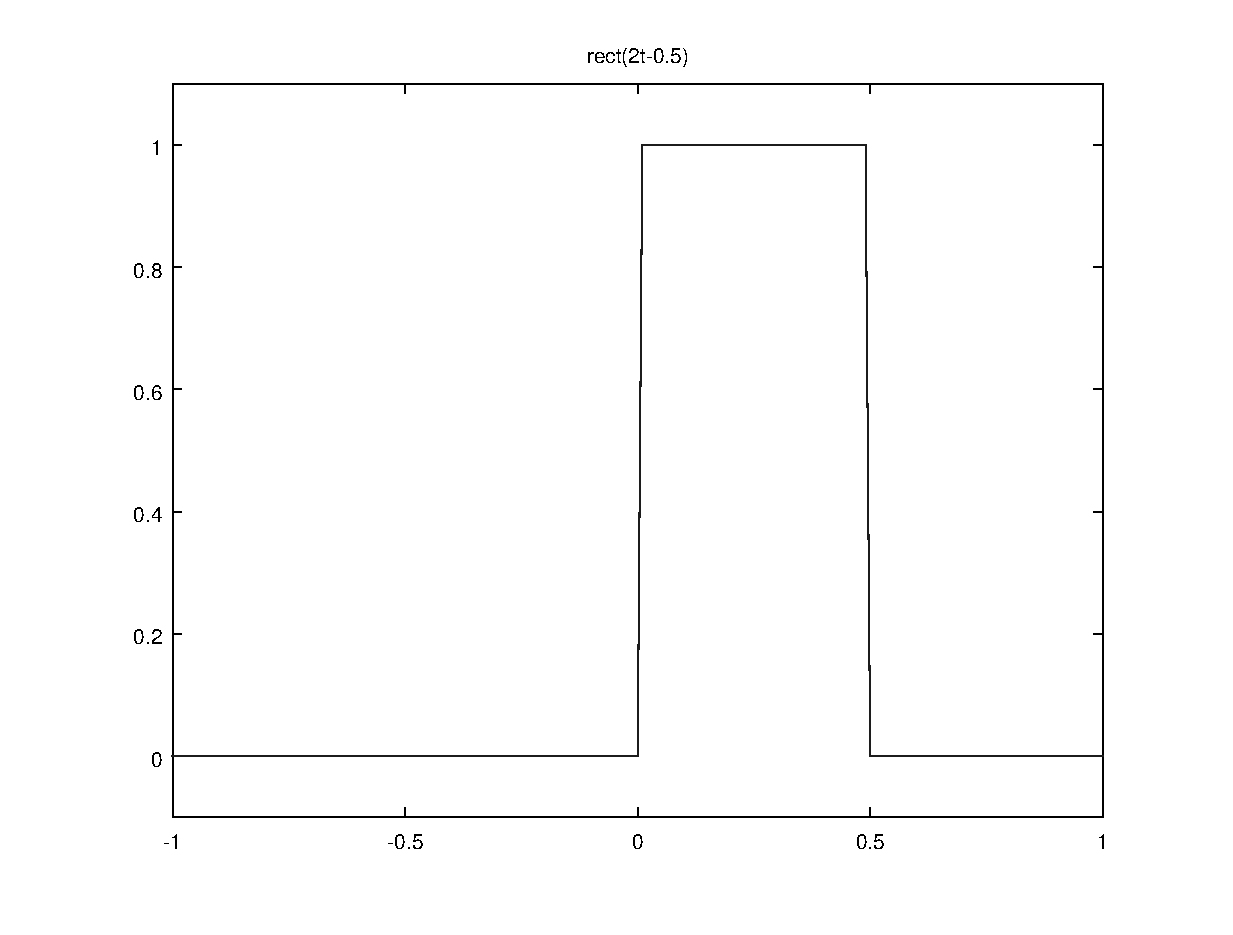
\includegraphics[width=0.6\textwidth]{rectA}
\caption{rect(2t - 0.5)}
\label{fig:rectA}
\end{figure}

\begin{equation*}
x(t)=rect((t-1)/2)+(t-1))
\end{equation*}

\begin{figure}[H]
\centering
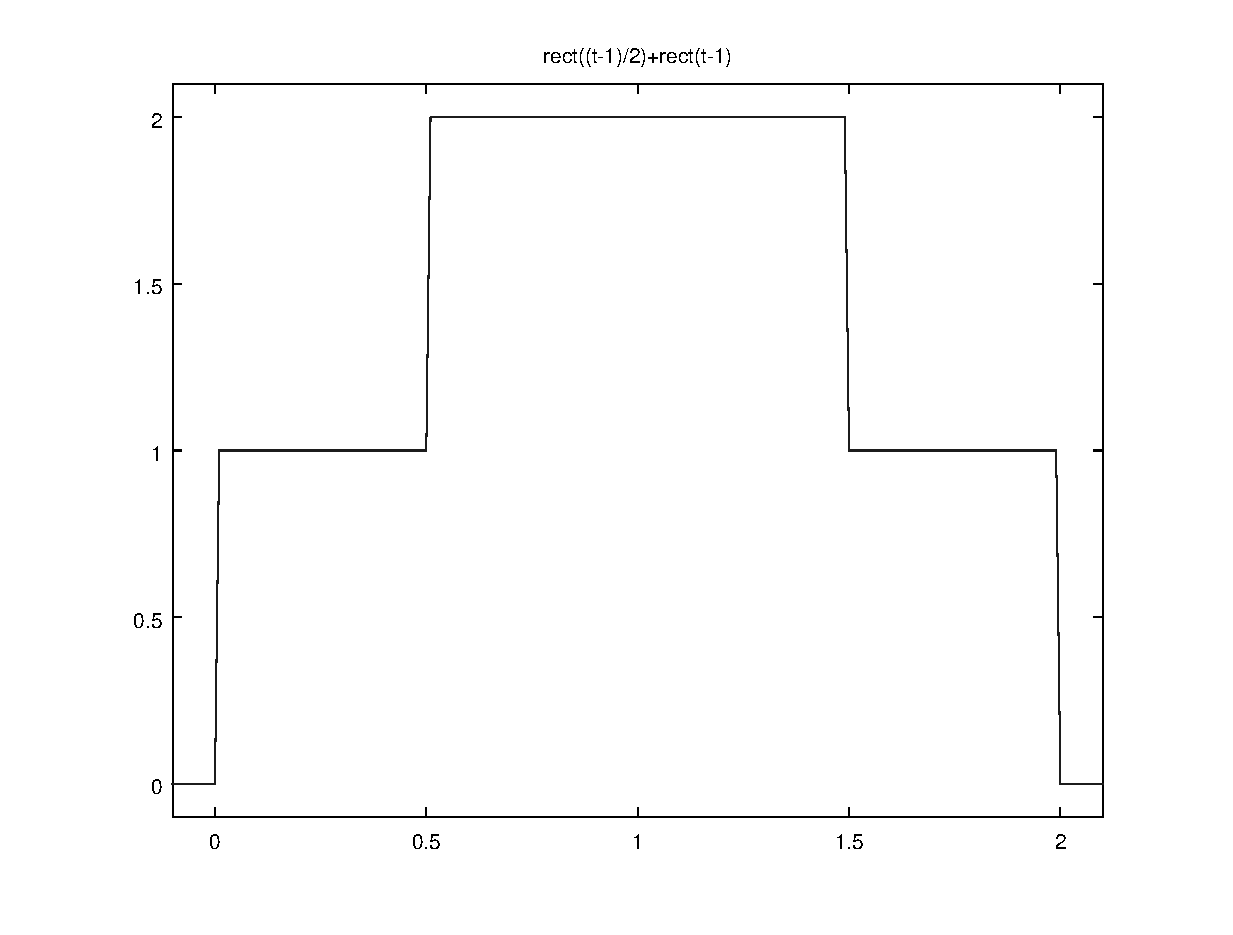
\includegraphics[width=0.6\textwidth]{rectB}
\caption{rect((t-1)/2)+(t-1)}
\label{fig:rectB}
\end{figure}








\section{Ejercicio 8}
Capture al menos dos señales físicas reales y preséntelas en una  gráfica e identifique el tipo de señal en algún segmento de la misma.\\

\begin{itemize}
\item La primera señal es un silbido humano.\\
Código de Matlab:\\
\begin{lstlisting}[frame=single]
>> [y,Fs] = audioread('Silb.wav');
>> sound(y,Fs);
>> figure(2);
>> plot(y);
\end{lstlisting}

\begin{figure}[htb]
\centering
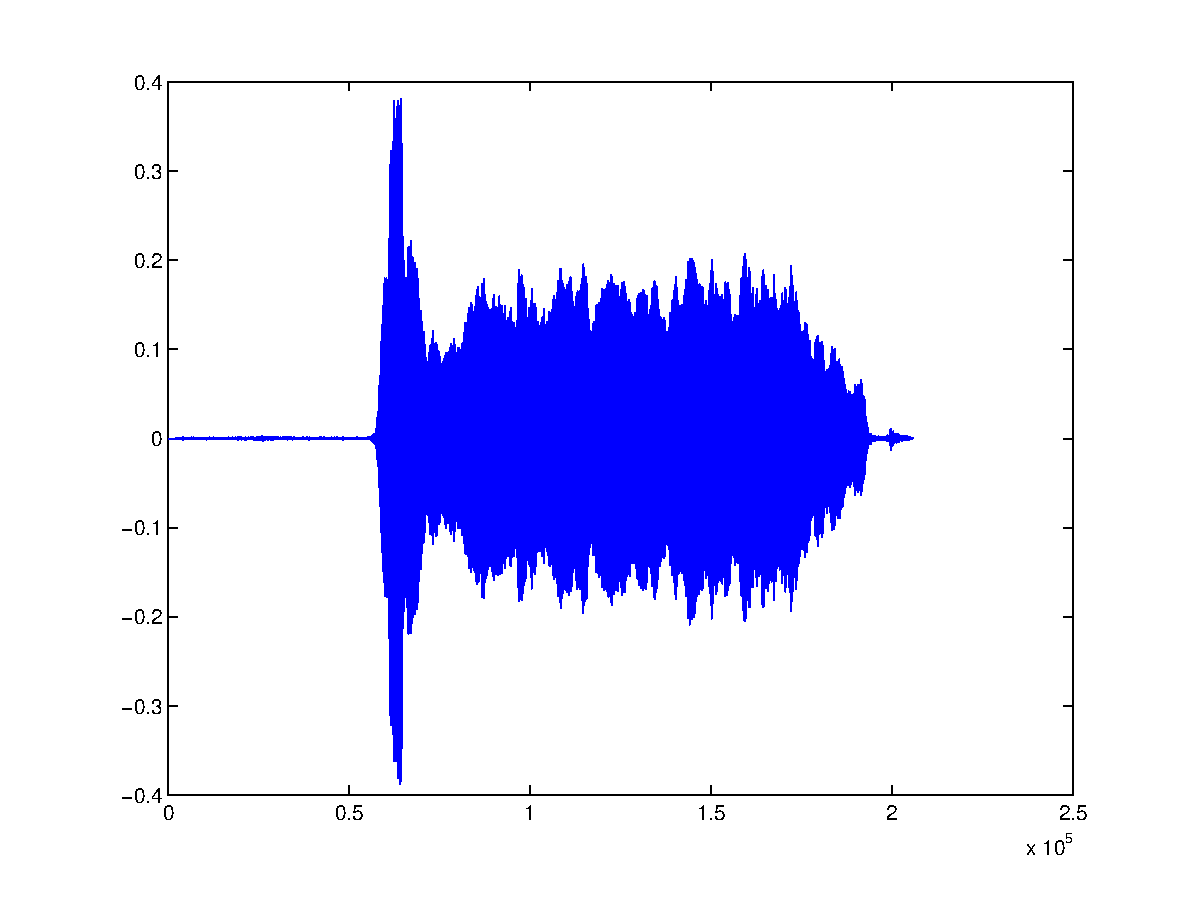
\includegraphics[width=0.6\textwidth]{SilbGraphic}
\caption{Silbido humano}
\label{fig:SilbGraphic}
\end{figure}

Esta es una señal de tiempo continuo por que la señal puede tomar cualquier valor en cualquier instante de tiempo. \\
Es una señal aperiódica, ya que no se repite en intervalos regulares \\
Es una señal aleatoria, ya que no se puede predecir mediante una función matemática.\\
Notamos en la gráfica que la señal el totalmente impredecible, ya que siempre parece tomar diferentes valores de frecuencia.

\item La segunda señal corresponde al sonido de las cuerdas de una guitarra acústica.\\
Código de Matlab:\\
\begin{lstlisting}[frame=single]
>> [y,Fs] = audioread('Guitar.wav');
>> sound(y,Fs);
>> figure(1);
>> plot(y);
\end{lstlisting}

\begin{figure}[H]
\centering
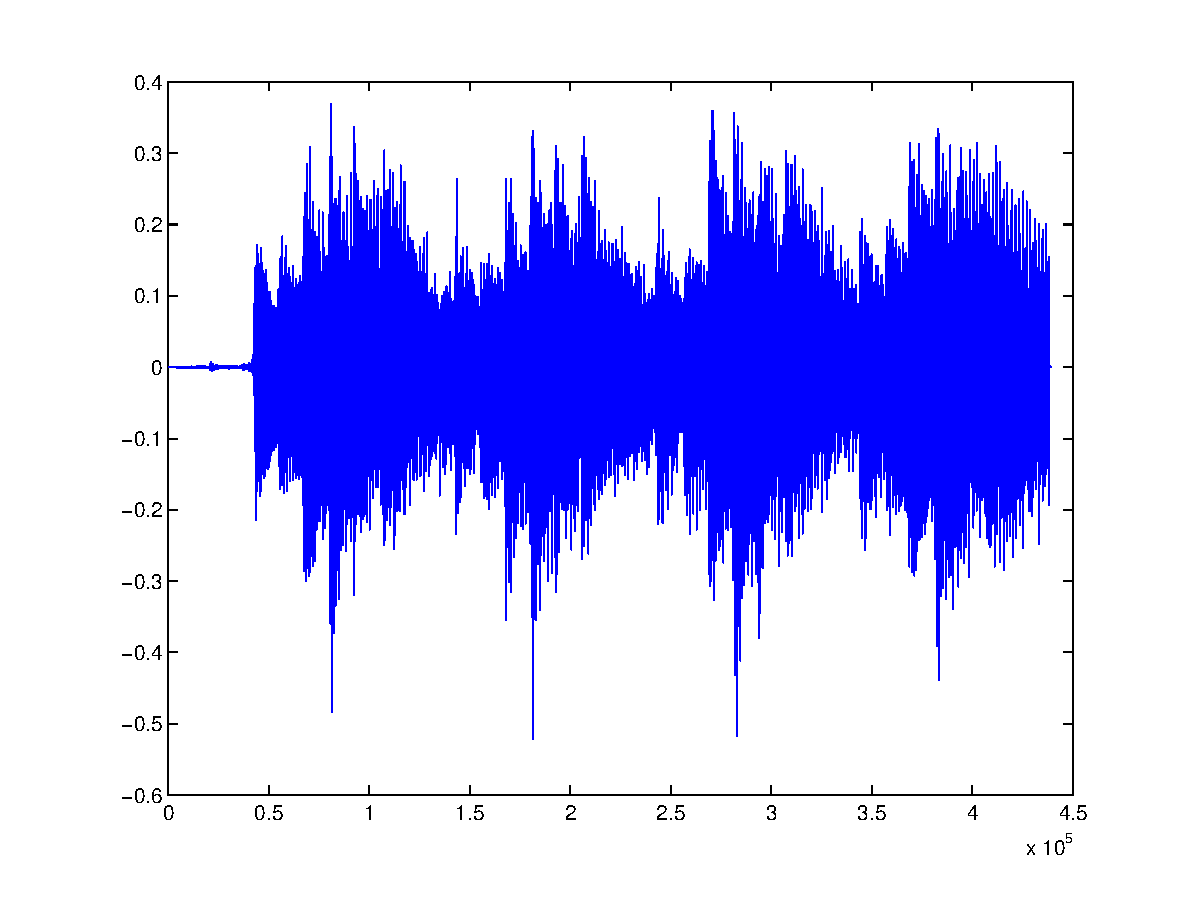
\includegraphics[width=0.6\textwidth]{GuitarGraphic}
\caption{Sonido de las cuerdas de una guitarra acústica}
\label{fig:GuitarGraphic}
\end{figure}

Esta es una señal de tiempo continuo por que la señal puede tomar cualquier valor en cualquier instante de tiempo. \\
Es una señal aperiódica, ya que no se repite en intervalos regulares \\
Es una señal aleatoria, ya que no se puede predecir mediante una función matemática.\\
NOTA: Se trató de que el rasgeo de las cuerdas de la guitarra sean igual en tiempo e intensidad, resultó un poco difícil, el mejor de los casos qes que hubiera salido igual la gráfica en intervalos regulares, para que la señal sea periódica y determinística.

\end{itemize}

\section{Ejercicio 9}

Conexión de sistemas en serie o cascada\\
\begin{equation}
S_{1}: y_{1}\left [ n \right ]=x_{1}\left [ n \right ]+2x_{1}\left [ n-1 \right ]
\end{equation}
\begin{equation}
S_{2}: y_{2}\left [ n \right ]=x_{2}\left [ n+2 \right ]+3x_{2}\left [ n \right ]
\end{equation}\\

S:\\
\begin{equation}
x_{2}\left [ n \right ]=y_{1}\left [ n \right ]=x_{1}\left [ n \right ]+2x_{1}\left [ n-1 \right ]
\end{equation}
\begin{equation}
x_{2}\left [ n+2 \right ]=x_{1}\left [ n+2 \right ]+2x_{1}\left [ n+2-1 \right ]
\end{equation}
\begin{equation}
3x_{2}\left [ n \right ]=3x_{1}\left [ n \right ]+(3)2x_{1}\left [ n-1 \right ]
\end{equation}\\

\begin{equation}
y\left [ n \right ]=y_{2}\left [ n \right ]=x_{1}\left [ n+2 \right ]+2x_{1}\left [ n+1 \right ]+3x_{1}\left [ n \right ]+6x_{1}\left [ n-1 \right ]
\end{equation}
\begin{equation}
y\left [ n \right ]=6x_{1}\left [ n-1 \right ]+3x_{1}\left [ n \right ]+2x_{1}\left [ n+1 \right ]+x_{1}\left [ n+2 \right ]
\end{equation}\\

Ahora sacaremos su sistema invertido\\
\begin{equation}
x_{1}\left [ n \right ]=y_{2}\left [ n \right ]=x_{2}\left [ n+2 \right ]+3x_{2}\left [ n \right ]
\end{equation}
\begin{equation}
x_{1}\left [ n \right ]=x_{2}\left [ n+2 \right ]+3x_{2}\left [ n \right ]
\end{equation}
\begin{equation}
2x_{1}\left [ n-1 \right ]=2x_{2}\left [ n-1+2 \right ]+(2)3x_{2}\left [ n-1 \right ]
\end{equation}\\

\begin{equation}
x\left [ n \right ]=x_{2}\left [ n \right ]=x_{2}\left [ n+2 \right ]+3x_{2}\left [ n \right ]+2x_{2}\left [ n+1 \right ]+6x_{2}\left [ n-1 \right ]
\end{equation}
\begin{equation}
x\left [ n \right ]=6x_{2}\left [ n-1 \right ]+3x_{2}\left [ n \right ]+2x_{2}\left [ n+1 \right ]+x_{2}\left [ n+2 \right ]
\end{equation}\\

Vemos que el sistema normal e invertido da el mismo resultado.

\section{Ejercicio 10}

Conexión de sistemas en serie o cascada\\

\begin{equation}
S_{1}: y_{1}\left [ n \right ]=nx_{1}\left [ n \right ]
\end{equation}
\begin{equation}
S_{2}: y_{2}\left [ n \right ]=x_{2}\left [ -n-1 \right ]
\end{equation}\\

S:\\

\begin{equation}
x_{2}\left [ n \right ]=y_{1}\left [ n \right ]=nx_{1}\left [ n \right ]
\end{equation}
\begin{equation}
x_{2}\left [ -n-1 \right ]=nx_{1}\left [ -n-1 \right ]
\end{equation}\\

\begin{equation}
y\left [ n \right ]=y_{2}\left [ n \right ]=nx_{1}\left [ -n-1 \right ]
\end{equation}
\begin{equation}
y\left [ n \right ]=nx_{1}\left [ -n-1 \right ]
\end{equation}\\

Ahora sacaremos su sistema invertido\\
\begin{equation}
x_{1}\left [ n \right ]=y_{2}\left [ n \right ]=x_{2}\left [ -n-1 \right ]
\end{equation}
\begin{equation}
nx_{1}\left [ n \right ]=nx_{2}\left [ -n-1 \right ]
\end{equation}
\begin{equation}
x\left [ n \right ]=nx_{2}\left [ -n-1 \right ]
\end{equation}\\

Vemos que el sistema normal e invertido da el mismo resultado.










\end{document}
